%!TEX root = ../thesis_main.tex
%!TEX encoding = UTF-8 Unicode
\vspace{-0.2cm}
\begin{flushright}
\emph{``The more data we have, the more likely we are to drown in it.''}\\
Nassim Nicholas Taleb, in \textit{Fooled by Randomness: The Hidden Role of Chance in Life and in the Markets}, 2008
\end{flushright}
\vspace{0.4cm}

Assessing the robustness of a roadmap driving the transition pathway of a whole-energy system is complex, especially due to the curse of dimensionality. This curse comes from the number of variables of the system (\eg the installed capacity of technologies), the multiple-year approach specific to the pathway optimisation (\ie versus the snapshot approach) or the number of uncertain parameters. On top of this, the sector coupling interconnecting the installed capacities and the used resources among the different (non-)energy sectors can make harder the understanding of big trends of such a system. To navigate through this load of uncertain and interconnected data, it is necessary to assess the robustness of pathway roadmaps.

To deal with such uncertainties, decision-makers have several options: (i) resistance; (ii) resilience; (iii) static robustness; and (iv) adaptive robustness \cite{walker2012deep}. Where resistance consists in planning for the worst-case scenario, resilience aims at a fast recovery whatever the conditions in the future. In static robustness, one seeks for a roadmap that would perform ``satisfactorily'' in a wide range of plausible futures, whereas, a roadmap would be dynamically robust if it is prepared to adapt in case of a change in conditions. The adaptability of the policy was addressed in Chapter \ref{chap:chap_RL}. The objective of this chapter is to apply the method described in Section \ref{sec:meth:PCA} to deal with the static robustness of pathway roadmaps.  \citet{castrejon2020making} assessed policy mix folllowing the same philosophy of ``satisfactory level of performance'' as \cite{walker2012deep}. In their work, they mostly focused on the electricity sector, accounting for a variety of stakeholders and related interests using STET (Socio-Technical Energy Transition) models to capture more properly societal and behavioral aspects in relation with policy implementation, enriching purely techno-economic model, like EnergyScope, that usually assume rational choice within an overall cost minimization.  However, in the case of the transition pathway of a whole-energy system, the challenges stand here in the definition of the ``performance metric'' as well as the ``satisfactory level of performance''. Between the total transition cost giving too few information and the entire set of installed technologies giving too much, the performance metric here is defined through the \gls{PCA} approach. Then, when comes the ``satisfactory level of performance'', we propose a relative level of performance through a comparative analysis of different roadmaps. Each roadmap will be ranked in terms of robustness.

\section*{Contributions}
\label{sec:RobPol:contributions}
The main contributions of this chapter is the application of the methodology proposed in Section \ref{sec:meth:PCA} to the case study of the Belgian energy transition. First, we apply the different steps that lead to the principal components of the transition. We analyse these big trends of variation and highlight the fact that these variations stand for the entire pathway, a group of consecutive representative years or rather on a tipping-year. Then, and most importantly, we assess the robustness of different technological roadmaps by projecting their resulting myopic pathway against these directions of variation. The application of \gls{PCA} to provide a new metric for robustness applied to the case of Belgium is the added-value of this chapter.

\section{Definition of the principal components of the transition}
\label{sec:RobPol:PC_transition}
The directions of variation, \ie the robustness metrics, are based on the installed capacities through the transition in the different end-use sectors, \ie electricity, \gls{HT} heat, \gls{LT} heat, passenger mobility, freight mobility, \gls{HVC}, ammonia and methanol (see Section \ref{subsec:meth:PCA:transition}). These capacities represent the technological roadmaps to supply these \gls{EUD} while respecting the \ce{CO2}-budget.  Data considered in this method come from the \gls{GSA} carried out on the perfect foresight optimisation of the Belgian transition pathway (see Chapter \ref{chap:atom_mol}). This gave 1260 different transitions resulting, for each of them, from the pathway optimisation subject to a sample of uncertain parameters (see Section \ref{subsec:uncert_charac}). Appendix \ref{app:UQ_tech_cap} gives the exhaustive distributions of the installed capacities among the different end-use sectors from the \gls{GSA}.

\subsection{Principal components of each representative year}
\label{subsec:RobPol:PC_year}
Before computing the \gls{PCs} of each representative year, we pre-preprocessed the raw data through scaling and managing the outliers (see Section \ref{subsec:meth:PCA:transition}). Managing the outliers is needed when assessing the main directions of variation of the transition. For example, decentralised \gls{HP} running on methane is discarded. This technology would have a contribution in the \gls{PCs} of transition for several reasons. First of all, the \gls{LT} heating sector represents between 22\% and 27\% of the \gls{EUD} in the case of Belgium. Being part of this major sector, the scaling of decentralised gas \gls{HP} is higher than technologies in other sectors. Then, given the \gls{LP} implementation of EnergyScope Pathway, the gas heat pumps completely substitute electric heat pumps in specific conditions (less electricity and cheaper methane). However, theses cases represent less than 10\% of the 1260 runs. For these reasons, we have decided that managing the outliers was needed to assess the main directions of variation of the transition.

The total variance decreases by more than 50\% between the earlier stages and the final ones (see Table \ref{tab:design_variance}). Even though the absolute value of these variances has no physical meaning, we observe that the variations are more important at earlier stages of the transition. In other words, the further the transition goes, the more limited the degrees of freedom are to respect the \ce{CO2}-budget.

\begin{table}[htbp]
\caption{Whole-system design variance of the different representative years and their comparison with 2025.} 
\label{tab:design_variance}
\centering
\begin{tabular}{c c c}
\toprule
\textbf{Year}      & \textbf{Design variance} [$10^{-3}$]	 &	\textbf{vs. 2025}\\
\midrule
2025 	&	$10.4$	& - 	\\
2030 	&	$12.1$	& +15\%	\\
2035 	&	$9.7$	& -7\% 	\\
2040 	&	$6.1$	& -42\% 	\\
2045 	&	$5.1$	& -51\% 	\\
2050 	&	$4.8$	& -54\% 	\\
\bottomrule
\end{tabular}
\end{table}

Then, keeping the \gls{PCs} capturing at least 90\% of the total variance of each representative year, this gives between four, in 2035, and seven, in 2050, \gls{PCs} depending on the year (see Figure \ref{fig:PC_over_the_years}), and a total of 34 \gls{PCs}. At later stages of the transition, the increasing number of required \gls{PCs}, in line with their smaller share of explained variance, is another indication that the variance of the system design is more spread over a wider range of technologies and with a more limited amplitude. 

\begin{figure}[!htbp]
\centering
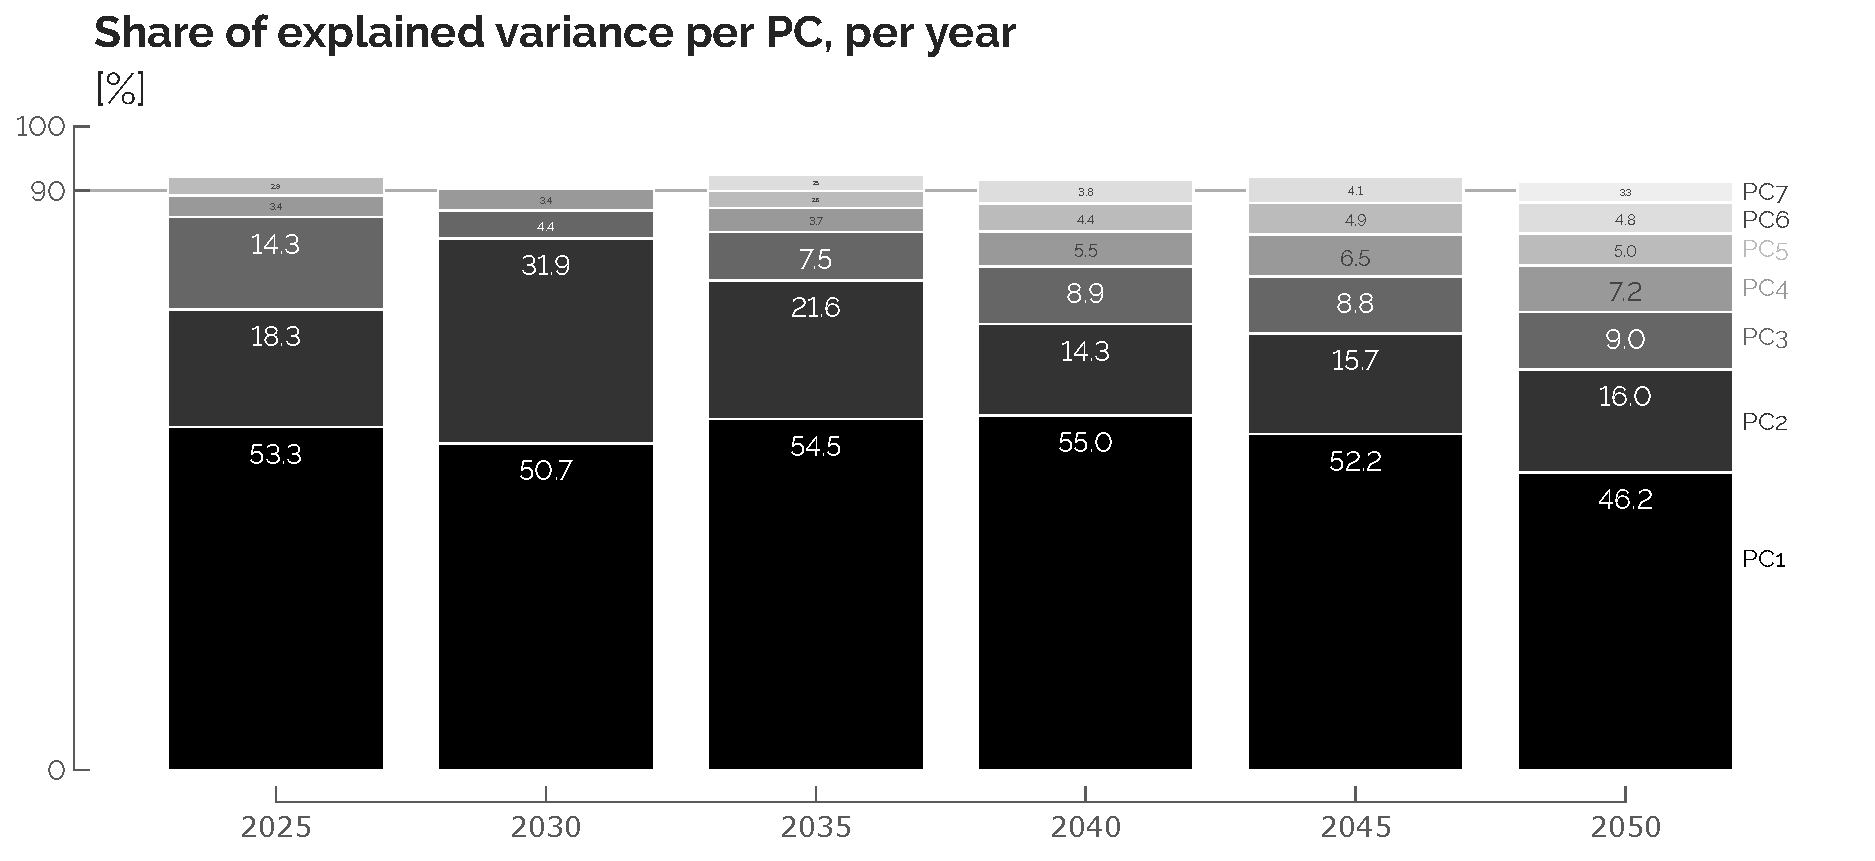
\includegraphics[width=\textwidth]{PC_over_the_years.pdf}
\caption{\gls{PCs} capturing at least 90\% of the total variance of their respective representative year of the transition. }
\label{fig:PC_over_the_years}
\end{figure}

Finally, we consider the respective contribution of the different technologies in the different $\text{PC}_{y}$, \ie their corresponding component in the different eigenvectors. Highlighting the top-5 technologies for $\text{PC}_{y,1}$, $\text{PC}_{y,2}$ and $\text{PC}_{y,3}$, we observe general trends over the whole transition as well as tipping year where there is a clear trade-off between several technologies (see Figure \ref{fig:Top5_PC_year}). The top-5 technologies of $\text{PC}_{y,1}$ represent on average 99.4\% of the norm of their respective PC. For $\text{PC}_{y,2}$ and $\text{PC}_{y,3}$, this share decreases to 97.6\% and 90.9\%, respectively.  As pointed out in Section \ref{subsec:meth:PCA:transition}, \gls{PCA} does not make any distinction between a vector of variation and its opposite. This is why $\text{PC}_{2025,1}$ and $\text{PC}_{2035,1}$ are actually very similar even though there are mostly on the opposite sides of the 0-axis.

\begin{figure}[!htbp]
\centering
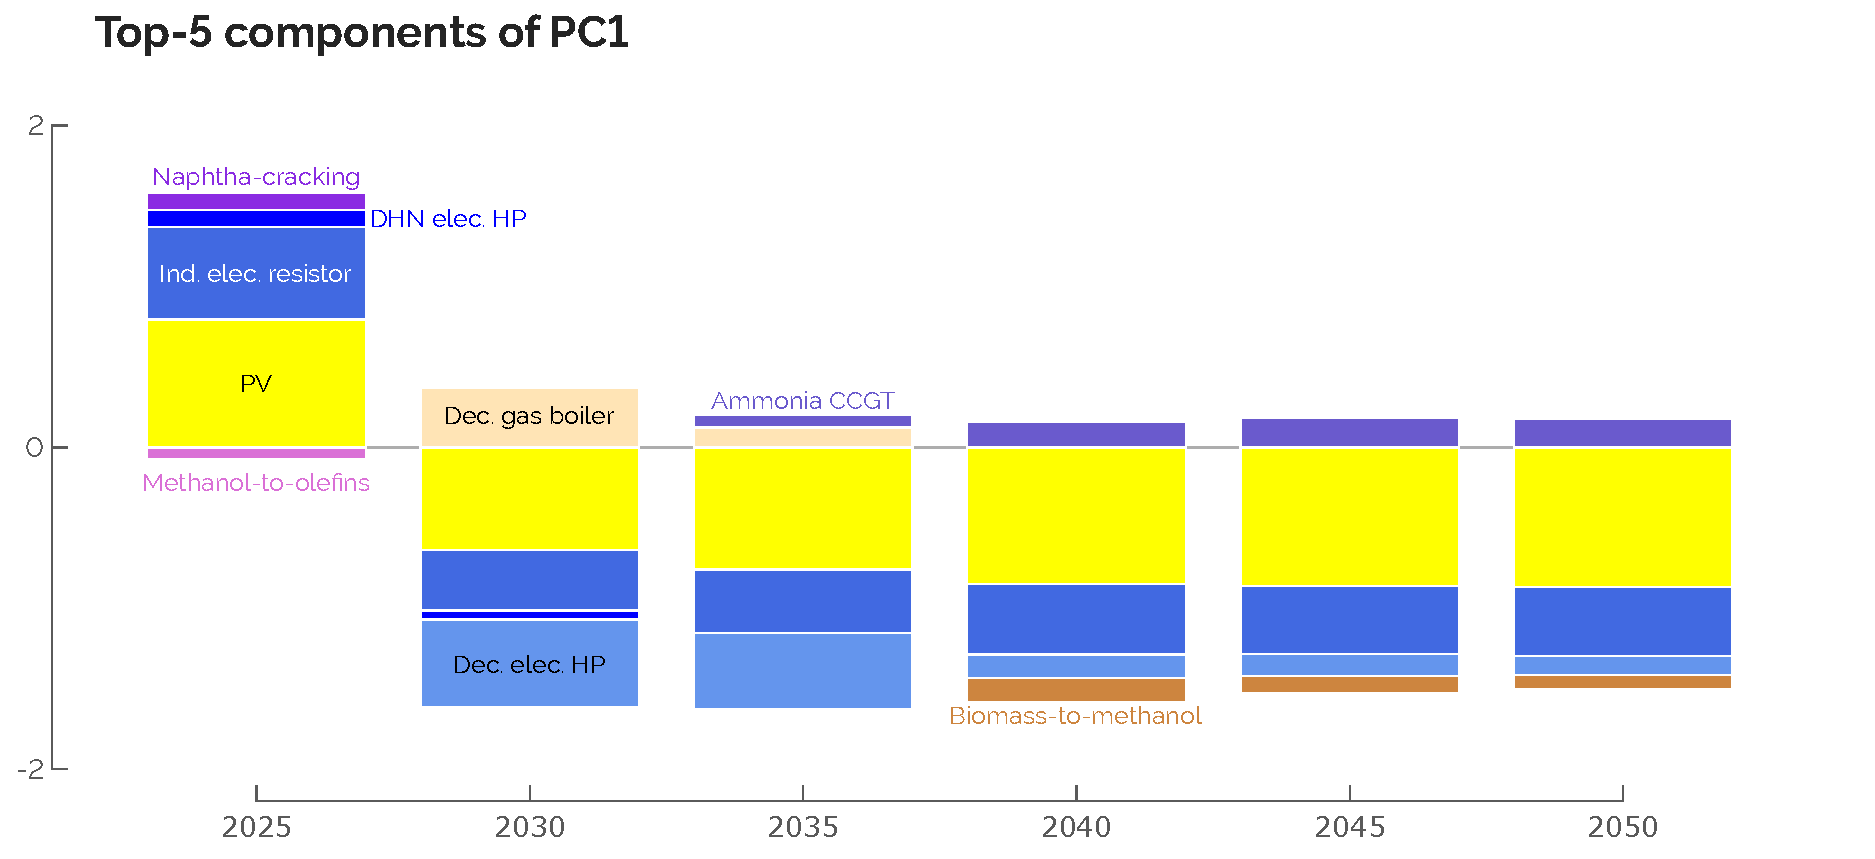
\includegraphics[width=0.9\textwidth]{Top5_PC1.pdf}
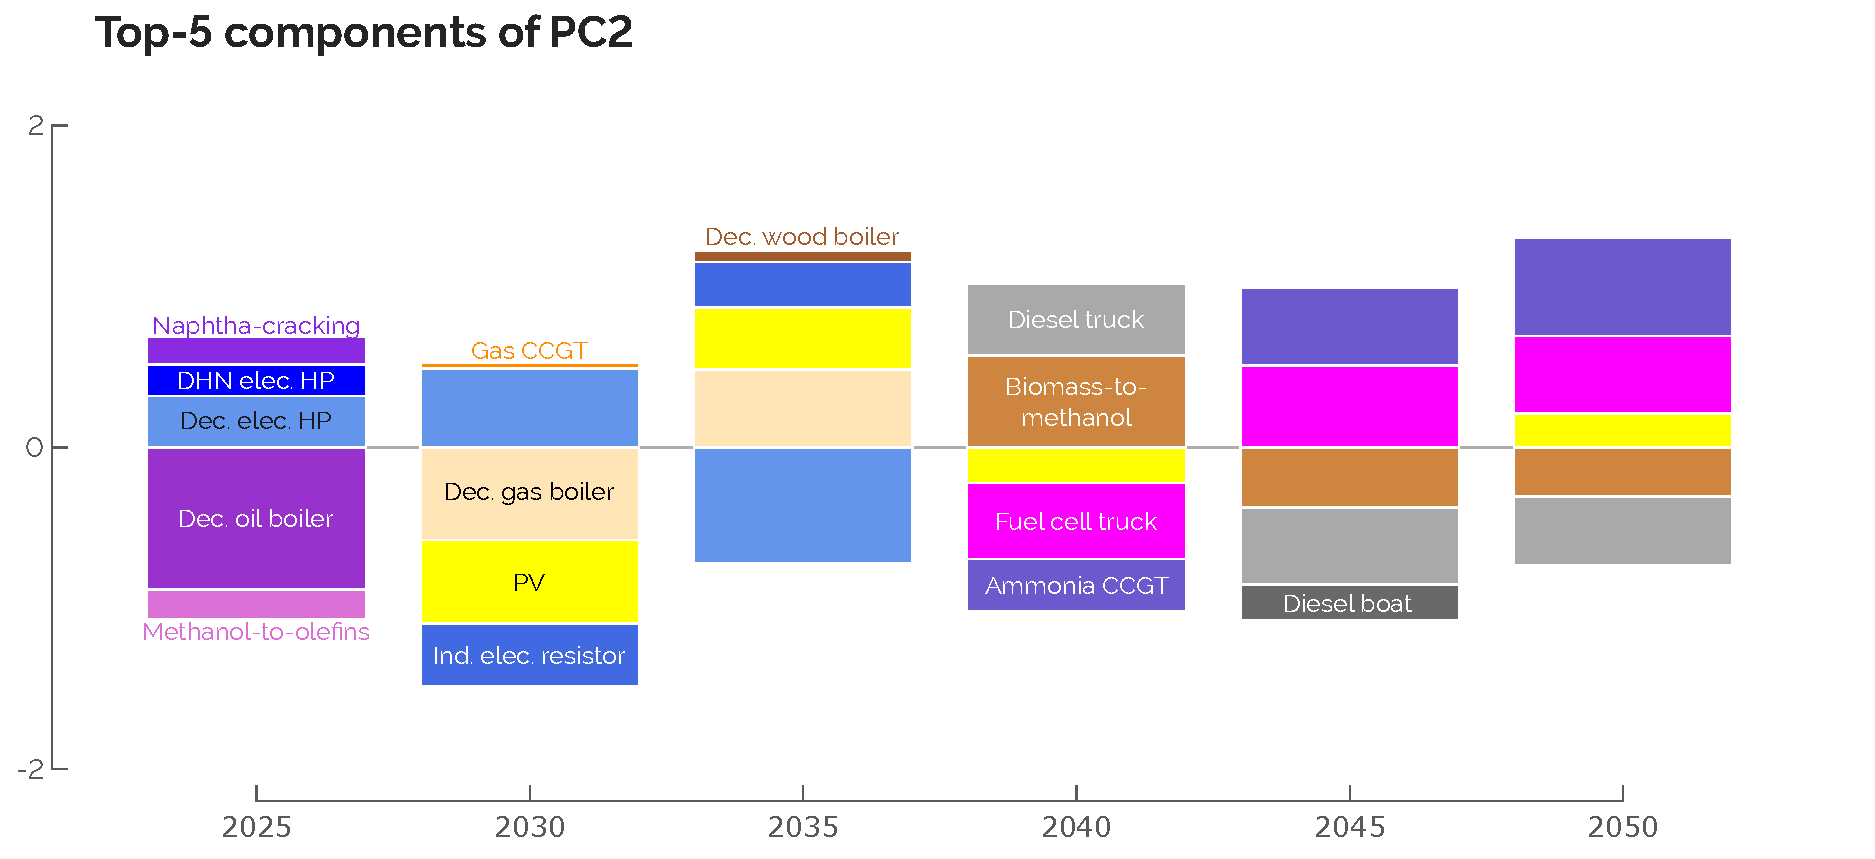
\includegraphics[width=0.9\textwidth]{Top5_PC2.pdf}
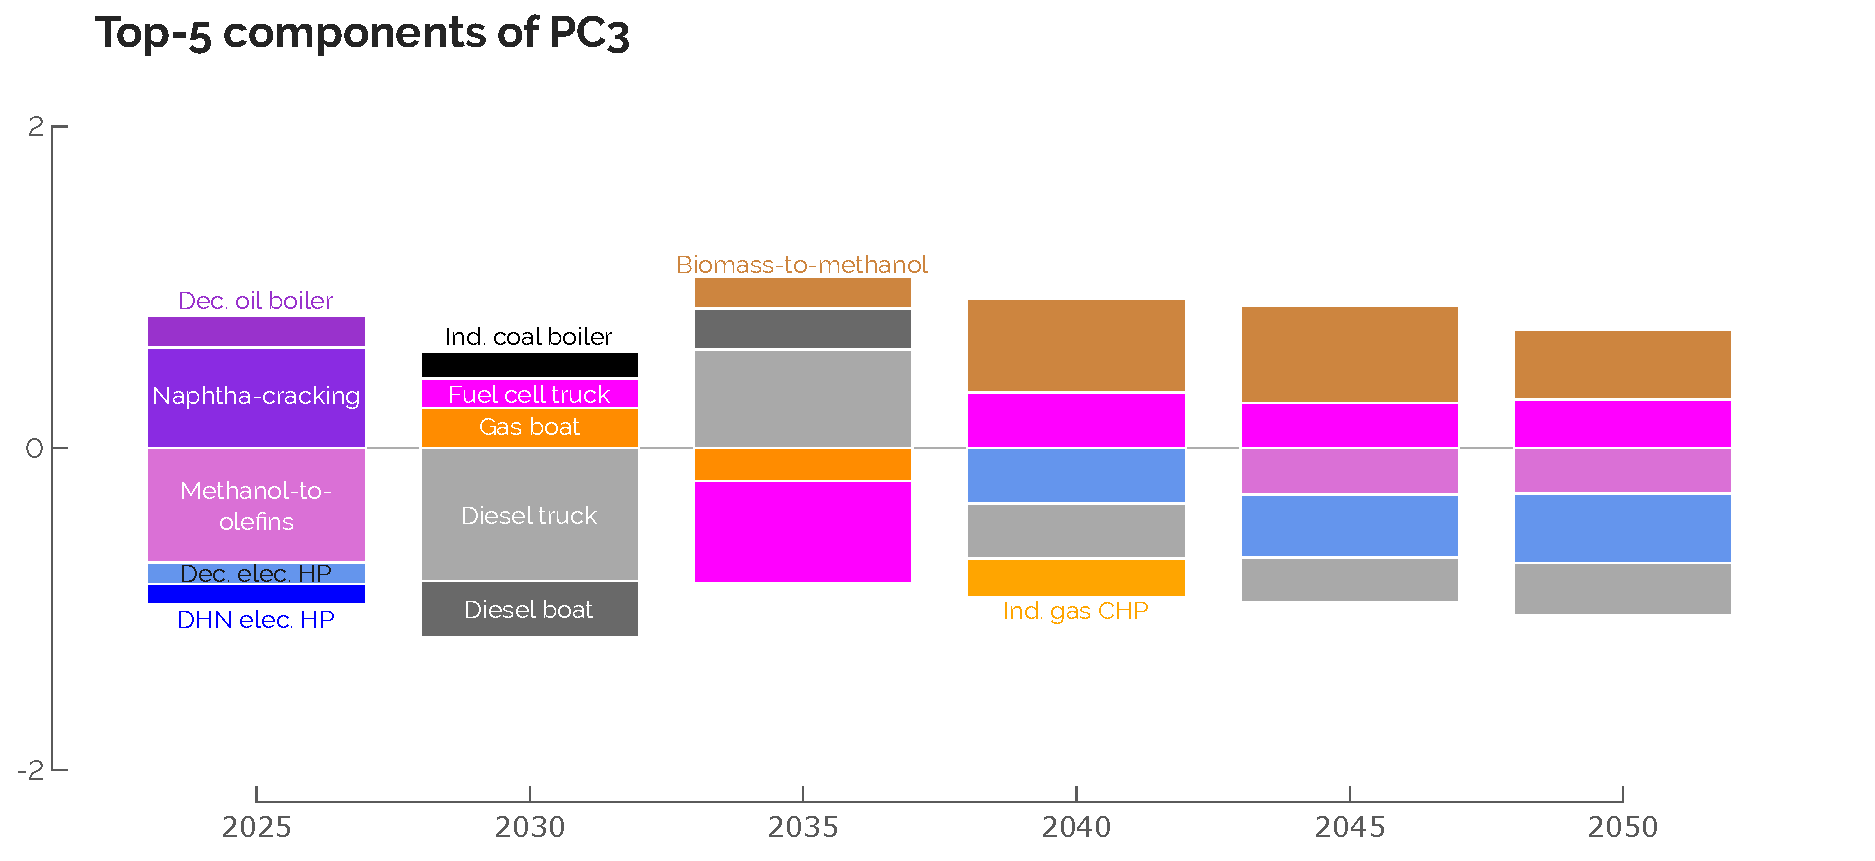
\includegraphics[width=0.9\textwidth]{Top5_PC3.pdf}
\caption{Contribution of the top-5 technologies to the first three \gls{PCs} over the different representative years. Where the variation of \gls{PV} panels supported by the electrification of the \gls{HT} heat via industrial electric resistors is the main varying drivers over the whole transition, there are tipping years like 2025 for the production of \gls{HVC} (\ie naphtha-cracker to \gls{MTO} or 2025-2030 for the production of \gls{LT} heat (\ie from oil and gas boilers to electric \gls{HP}.}
\label{fig:Top5_PC_year}
\end{figure}

Even though the following observations could be made by analysing the distribution of installed capacities (see Appendix \ref{app:UQ_tech_cap}) or the covariance matrices, the \gls{PCA} decomposition offers a more visual and summarising representation of the main trends of variation. Due to their intermittency, increasing the integration of \gls{PV} panels requires the installation of other technologies to benefit from free and renewable electricity when it exceeds the electrical \gls{EUD}. Therefore, we observe that the variation of installed \gls{PV} is directly linked with the variation of installed industrial electrical resistors and, to a smaller extent, of decentralised and \gls{DHN} electrical \gls{HP}. These variations spread over the whole transition and they are the main varying factors to the first $\text{PC}_{\text{transition}}$. Where this was an example for correlated technologies, we can also identify some key modal shifts where one technology is either substituted or in balance with others. First, about the \gls{LT} heat sector, the early stages of the transition, \ie 2025-2030, sees the shift from mainly decentralised oil and gas boilers towards decentralised and \gls{DHN} electrical \gls{HP}. Later in the transition, there seems to be a tight competition between (bio)diesel and \gls{FC} trucks that drive the design variance to a smaller extent as they mostly appear in the second and third \gls{PCs} of the representative years. Representing a smaller share of the total variance, there are other modal shifts (\eg \gls{BEV} substituting diesel and gasoline cars) that are not visible through the \gls{PCs}. Besides these modal shifts spread over several representative years, 2025 is the tipping year concerning the shift from naphtha-cracker to methanol-to-olefins to supply \gls{HVC}. Finally, there are also technologies contributing to \gls{PCs} because they are the main producing assets of their respective end-use sector and the demand varies significantly, \eg biomass-to-methanol.

\subsection{Principal components of the perfect foresight REF transitions}
\label{subsec:RobPol:PC_transition}
Based on the \gls{PCs} of each representative year (34 in total), this section identifies a sufficient subset to characterise the roadmaps (and assess their robustness in Section \ref{subsec:RobPol:Projection}).

Before aggregating and averaging similar $\text{PC}_{y}$, it is necessary to rank them to ensure capturing most of the transition variance in the subsequent $\text{PC}_{\text{transition}}$.This ranking is based on the design variance captured by each $\text{PC}_{y}$ in their respective representative year (see Table \ref{tab:ranking_PCs}). Summing all of these variances over the different years results in a ``pseudo'' total variance of the transition. To construct the \gls{PCs} of the transition, $\text{PC}_{\text{transition}}$, we keep the $\text{PC}_{y}$ that captures at least 85\% of this total variance of the transition (see Section \ref{subsec:meth:PCA:transition}).  This results in keeping 14 $\text{PC}_{y}$: the first and second \gls{PCs} of each representative year and the third PC of 2025 and 2035. 

\begin{table}[htbp!]
\caption{Ranking of \gls{PCs} per design variance captured in their respective representative year and cumulative share of the captured total variance of the transition}
\label{tab:ranking_PCs}
\centering
\begin{tabular}{c c c c c}
\toprule
\multirow{2}{*}{\textbf{Ranking}} & \multirow{2}{*}{\textbf{Year}}  & \multirow{2}{*}{\textbf{PC}} & \multirow{2}{*}{\textbf{Design variance} [$10^{-4}$]} & \textbf{Cumulative share of} \\	
 &   &  &  & \textbf{total variance} [\%] \\	
 \midrule	
1 & 2030 & $\text{PC}_1$ & 61.1 & 13.9 \\
2 & 2025 & $\text{PC}_1$ & 55.7 & 26.5 \\
3 & 2035 & $\text{PC}_1$ & 52.7 & 38.4 \\
4 & 2030 & $\text{PC}_2$ & 38.4 & 47.2 \\
5 & 2040 & $\text{PC}_1$ & 33.4 & 54.7 \\
6 & 2045 & $\text{PC}_1$ & 26.5 & 60.7 \\
7 & 2050 & $\text{PC}_1$ & 22.2 & 65.8 \\
8 & 2035 & $\text{PC}_2$ & 20.9 & 70.5 \\
9 & 2025 & $\text{PC}_2$ & 19.1 & 74.8 \\
10 & 2025 & $\text{PC}_3$ & 15.0 & 78.2 \\
11 & 2040 & $\text{PC}_2$ & 8.7 & 80.2 \\
12 & 2045 & $\text{PC}_2$ & 7.9 & 82.0 \\
13 & 2050 & $\text{PC}_2$ & 7.7 & 83.7 \\
14 & 2035 & $\text{PC}_3$ & 7.3 & \textbf{85.4} \\
$\vdots$ & $\vdots$ & $\vdots$ & $\vdots$ & $\vdots$\\
34 & 2050 & $\text{PC}_7$ & 1.6 & 100 \\
\bottomrule							

\end{tabular}
\end{table}

Given the similarity between $\text{PC}_y$ (see Figure \ref{fig:Top5_PC_year}), some $\text{PC}_{\text{transition}}$ result from the aggregation and averaging of the components of several $\text{PC}_y$ (see Table \ref{tab:PC_transition_aggregation}). This aggregation step has a double objective: limiting the dimension of the robustness metrics and avoiding ineffective redundancy in terms of $\text{PC}_{\text{transition}}$ where several of them would otherwise point towards similar directions of variation.

\begin{table}[htbp!]
\caption{Aggregation of $\text{PC}_y$ to construct the $\text{PC}_{\text{transition}}$ and share of the captured total variance of the transition by each $\text{PC}_{\text{transition}}$.}
\label{tab:PC_transition_aggregation}
\centering
\begin{tabular}{c c c}
\toprule
 \multirow{2}{*}{$\mathbf{\textbf{PC}_{\textbf{transition}}}$} & \multirow{2}{*}{$\mathbf{\textbf{PC}_{\textbf{y}}}$} & \textbf{Share of total} \\	
 &  & \textbf{variance} [\%] \\	
 \midrule
\multirow{6}{*}{$\text{PC}_{\text{transition,1}}$} & $\text{PC}_{\text{2025,1}}$ & \multirow{6}{*}{57.0}\\
& $\text{PC}_{\text{2030,1}}$ & \\
& $\text{PC}_{\text{2035,1}}$ & \\
& $\text{PC}_{\text{2040,1}}$ & \\
& $\text{PC}_{\text{2045,1}}$ & \\
& $\text{PC}_{\text{2050,1}}$ & \\
 \midrule
\multirow{2}{*}{$\text{PC}_{\text{transition,2}}$} & $\text{PC}_{\text{2030,2}}$ & \multirow{2}{*}{13.4}\\
& $\text{PC}_{\text{2035,2}}$ & \\
\midrule
\multirow{4}{*}{$\text{PC}_{\text{transition,3}}$} & $\text{PC}_{\text{2040,2}}$ & \multirow{4}{*}{7.2}\\
& $\text{PC}_{\text{2045,2}}$ & \\
& $\text{PC}_{\text{2050,2}}$ & \\
& $\text{PC}_{\text{2035,3}}$ & \\
 \midrule
$\text{PC}_{\text{transition,4}}$ & $\text{PC}_{\text{2025,2}}$ & 4.3\\
 \midrule
$\text{PC}_{\text{transition,5}}$ & $\text{PC}_{\text{2025,3}}$ & 3.4\\
\bottomrule							

\end{tabular}
\end{table}

\newpage
Averaging the components of similar $\text{PC}_y$ allows constructing the $\text{PC}_{\text{transition}}$ (see Figure \ref{fig:Top5_PC_transition}). These directions of variation form the robustness matrix on which it is possible to project the results of transition roadmaps tested under uncertainties and myopic pathway optimisation.

\begin{figure}[!htbp]
\centering
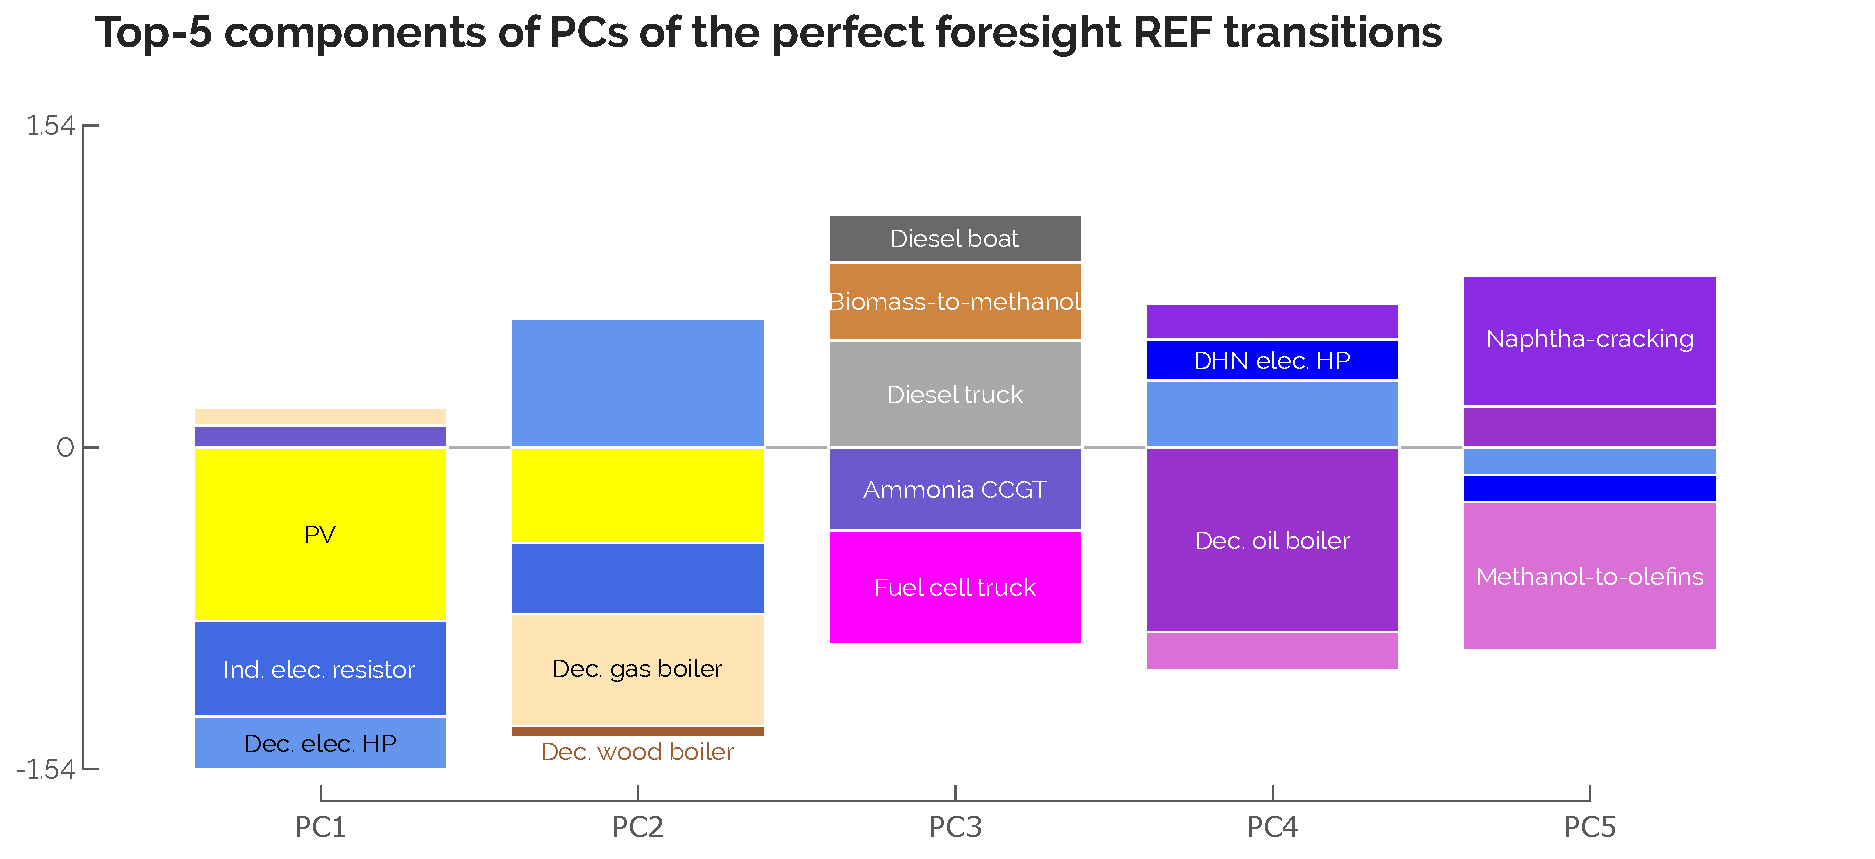
\includegraphics[width=0.8\textwidth]{Top5_PCtransition.pdf}
\caption{Contribution of the top-5 technologies to the different $\text{PC}_{\text{transition}}$. }
\label{fig:Top5_PC_transition}
\end{figure}

\newpage
\section{Robustness assessment of pathway roadmaps}
\label{sec:RobPol:Rob_Assessment}
Now that the performance metric is defined, we can assess the robustness of different roadmaps. These roadmaps are defined as the technological mix given by the deterministic optimisation of the perfect foresight pathway under certain conditions. The two first roadmaps are the \textbf{REF} and \textbf{SMR} cases (see Chapter \ref{chap:atom_mol}). All the uncertain parameters are considered at their nominal value in these two cases. The only difference consists in allowing \gls{SMR} from 2040 onward in the \textbf{SMR} case. On top of these two cases, we add a so-called ``robust'' case, \textbf{ROB}, in the same sense as in the works of \citet{bertsimas2004price} or \citet{Moret2017PhDThesis} accounting for a ``protection parameter''. Then, we assess the robustness of these three roadmaps via a ``three-step rolling horizon approach'' extended from the work of \citet{moret2020overcapacity}: (i) setting the initial investment strategies provided by the roadmaps and, (ii) assessing the variation of additional investments needed through myopic pathway optimisation under uncertainties and, (iii) projecting the strategies from the myopic optimisations on the robustness metrics defined via \gls{PCA}. Finally, we assess the variation of the transition costs resulting from these myopic transitions under uncertainties.

\subsection{A robust roadmap?}
\label{subsec:RobPol:Rob_roadmap}
Rather than considering all the uncertain parameters at their worst values as in the work of \citet{soyster1973convex}, we follow here the robust approach of \citet{bertsimas2004price} and \citet{Moret2017PhDThesis}. In their works, the authors consider a factor $\Gamma_{\text{obj}}\in [0,d]$ that represents a ``protection parameter'' of the objective function where $d$ is the total number of uncertain parameters (see Section \ref{subsec:pce}). If $\Gamma_{\text{obj}}= 0$, where all the uncertain parameters are at their nominal value, we obtain the deterministic solution of the \textbf{REF} case. If $\Gamma_{\text{obj}}= d$, this means considering the ``fully robust'' solution where all the uncertain parameters are their worst value, as in \citet{soyster1973convex}.  Between these two extreme cases, the uncertain parameters to account for at their worst values follow the ranking given by the \gls{GSA} (see Chapter \ref{chap:atom_mol}). In practice, $\Gamma_{\text{obj}}= 1$ means considering the cost of purchasing electrofuels at its worst value. $\Gamma_{\text{obj}}= 2$ adds the industry \gls{EUD} at its worst value, and so on. In the present analysis, we label the roadmap as ``robust'' (ROB) by setting $\Gamma_{\text{obj}}= 6$. Consequently, the following six parameters are set at their worst value (upper bound of their range): costs of purchasing electrofuels, fossil fuels and biofuels as well as the industry \gls{EUD}, the interest rate and the variable OPEX of technologies. In practice, this means that, in the ROB case, imported energy carriers, except electricity, are 179.8\% more expensive, the industrial demand is, by 2050, 23.9\% higher\footnote{As detailed in Chapter \ref{chap:case_study}, the industrial demand encompasses the whole \gls{NED} and \gls{HT} heat demand, as well as the industrial share of electricity and \gls{LT} heat demands.}, the interest rate is increased by 46.2\% (\ie 2.2\% versus 1.5\% in the REF case) and the variable OPEX of technologies, $c_{\text{\emph{maint}}}$, is 35.7\% higher. 

Besides the additional operational costs due to more expensive energy carriers, this case presents cumulative investments over the transition that are 2.6\% (17\,b€) higher than the REF case. The following paragraphs investigate the differences in the different sectors between the ROB and the REF cases, similarly to the comparison carried out with the SMR case in Chapter \ref{chap:atom_mol}.\\

\myparagraph{Power sector}\\

Given the more expensive imported energy carriers, the model opts for an earlier electrification of the system and more efficiency. Consequently, the power sector is one of the most impacted ones (see Figure \ref{fig:rob_pol_ROB_elec}). At the earlier stages of the transition,  the model opts for the full deployment of local \gls{VRES} as soon as possible and importing more electricity (\ie +8.7~TWh, +52\%) from abroad in 2025.  This earlier and bigger integration of \gls{VRES} is supported by the higher electrification of \gls{HT} and, to a smaller extent the \gls{LT}, heating sector as well as in the mobility sectors. It is mostly the industrial electric heaters that absorb the abundant and intermittent electricity produced by \gls{PV} panels and wind turbines. In the mobility sectors, \gls{BEV} substitutes gasoline cars from 2025 onward and electric trucks substitute diesel trucks in the near-term before being substituted by \gls{FC} trucks at the end of the transition.  On the supply side, besides the local \gls{VRES} and the direct import of electricity from abroad, \gls{CHP} units, mostly industrial, are favoured given their higher efficiency at the expense of ammonia-\gls{CCGT}. In the ROB case, by 2050, these \gls{CHP} units produce 43.3~TWh, \ie 23\% of the total electricity production, versus 21.9~TWh in the REF case. These observations are in line with the work of  \citet{moret2020overcapacity} focusing on the problem of overcapacity in the European power sector. The authors highlighted that the robust strategy diversified the supply sources of electricity between \gls{VRES}, import of electricity and more efficient technologies like \gls{CHP} and \gls{HP}.

\begin{figure}[htbp!]
\centering
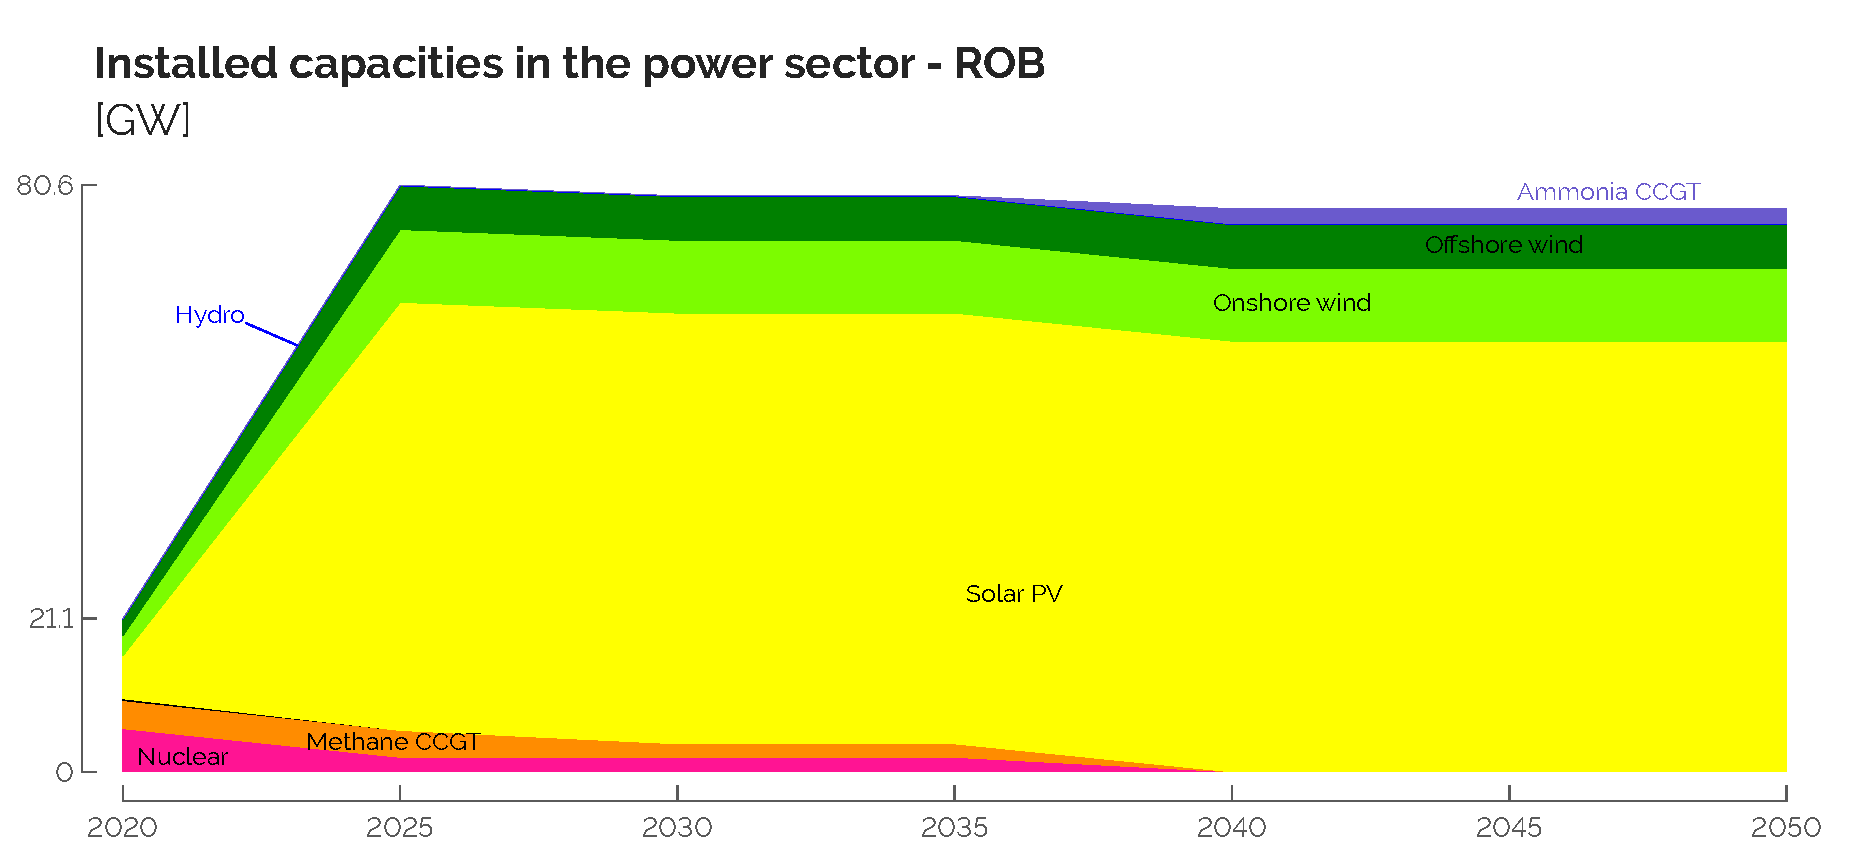
\includegraphics[width=0.82\textwidth]{Elec_Tech_Cap_ROB.pdf}
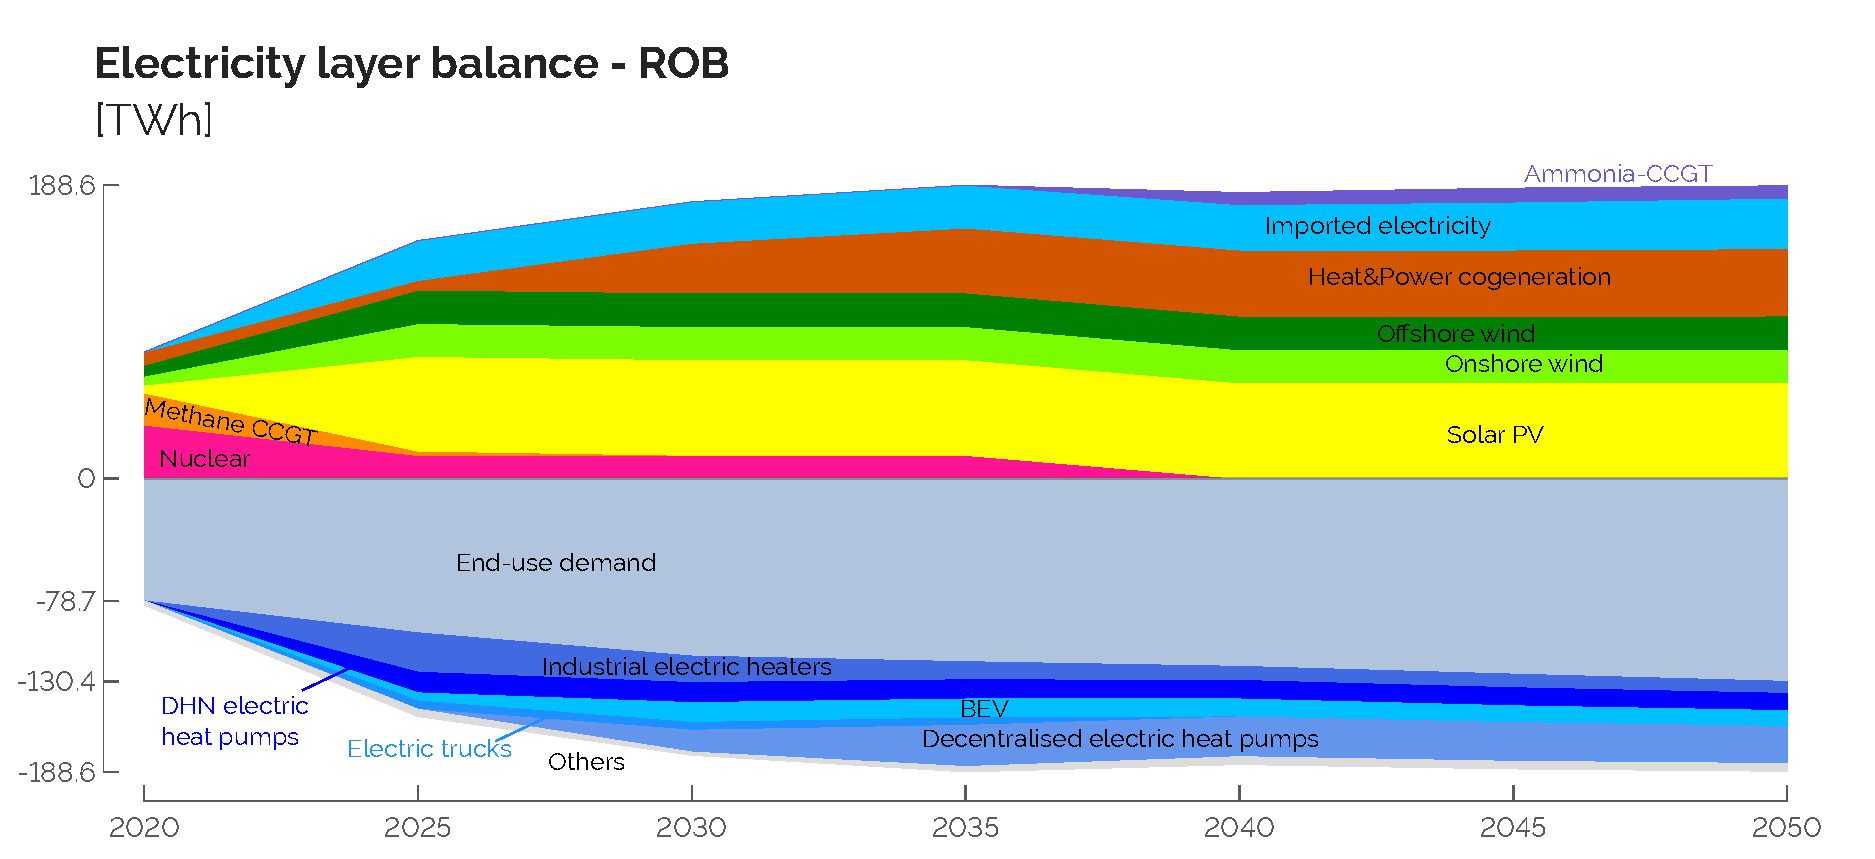
\includegraphics[width=0.82\textwidth]{Elec_Layer_ROB.pdf}
\caption{Installed capacities and layer balance of the power sector in the ROB case. Compared to the REF case, local \gls{VRES} are deployed as soon as possible supported by an earlier electrification of the heat and transport sectors. \gls{CHP} units also represents a higher share of the electricity supply given their higher efficiency at the expense of other flexible production units like ammonia-\gls{CCGT}.}
\label{fig:rob_pol_ROB_elec}
\end{figure}

\myparagraph{Heating sectors}\\

By 2050, the additional 23.9\% of industrial \gls{EUD} directly impacts the technological mix to supply the \gls{HT} heat, \ie +13.6~TWh as direct \gls{HT} heat \gls{EUD} on top of the extra 3.4~TWh consumed by the \gls{MTO} process. As aforementioned, at earlier stages of the transition, up to 20.9~GW of industrial electric heaters supply the additional demand and support the integration of solar \gls{PV}.  However, in the mid-term, 27\% of these heaters are prematurely decommissioned where 24\% are not renewed after reaching the end of their lifetime. Instead, up to +3.5~GW of industrial \gls{CHP} units are installed to efficiently use e-methane that is considered more expensive in the ROB case to supply electricity and 52\% of the \gls{HT} heat demand. About the \gls{LT} heat sector, the principal impact is the bigger installation of \gls{DHN} and decentralised electric \gls{HP}, up to +2.1~GW and +0.8~GW respectively. \\

\myparagraph{Mobility sectors}\\

In the ROB roadmap, the transport of freight by trucks first transitions from diese to electric trucks and then, after 2035, to \gls{FC} trucks. Used as a way to support the the early installation of solar \gls{PV}, electric trucks are then replaced by \gls{FC} ones given the limited availability of renewable electricity and its more cost-effective use in other sectors such as private mobility. Freight transport via trains and boats are not different from the REF roadmap. About the passenger mobility, compared to the REF case, the shift from \gls{ICE} cars to \gls{BEV} occurs earlier in the transition, in line with the increased production of intermittent electricity from \gls{VRES}. \\

\myparagraph{Non-energy}\\

Technologically speaking, by 2050, the ROB case accounts for an additional 1.2~GW of \gls{MTO} to supply the extra 10.3~TWh of \gls{HVC}. Besides this, the extra 2.5~TWh and 0.4~TWh of e-ammonia and e-methanol are supplied by the import of their respective energy carrier.\\

In conclusion, the two main assumptions impacting the ROB roadmap strategy compared to the REF one were the higher cost of purchasing imported energy carriers (except electricity) and higher industrial \gls{EUD}. More expensive imported energy carriers lead to an earlier full deployment of local \gls{VRES} (\ie \gls{PV}, wind onshore and offshore) and an increase of the share of the total OPEX due to the consumption of resources (\ie excluding the OPEX of the technologies) in the total transition cost: \ie 56\% versus 38\% in the REF case. This, combined with the increase of industrial \gls{EUD}, encourages a more efficient use of the resources, \ie \gls{CHP} and \gls{HP}. The increased interest rate and variable OPEX of technologies have a more negligible impact on the roadmap strategy as they identically affect the entire set of technologies.

\subsection{Projection on robustness metric}
\label{subsec:RobPol:Projection}
After defining the robustness metric and describing the roadmaps to assess (\ie REF, SMR and ROB), the final step consists in testing these roadmaps under uncertainties in myopic pathway optimisations. This aims at assessing the adaptation of the roadmaps as uncertainty gradually unfolds over time \cite{moret2020overcapacity}, which brings more realism than perfect foresight \cite{poncelet2016myopic}. The three roadmaps are tested 500 times fixing the installed capacities $f_{\mathrm{max}}\geq\textbf{F}\geq\textbf{F}^*$ for all the end-use technologies, and taking values of the 34 uncertain parameters (see Section \ref{sec:cs:uncertainty}) following the Sobol' sequence. However,  some uncertain parameters limit the potential installed capacity, $f_{\mathrm{max}}$, of \gls{PV} panels, onshore and offshore wind turbines and \gls{SMR}. For these, in case the installed capacity prescribed by the roadmap is higher than the maximum potential affected by the value of the uncertain parameter, the actual installed capacity is set to this new limit. In reality, this would be similar to revise to a smaller extent the expected roadmap due to external events (\eg smaller public acceptance \cite{zoellner2008public,sam2014small}, lower \gls{TRL} or longer installation time than expected).

The SMR roadmap spans over similar ranges as the REF case (see Table \ref{tab:projection}). The most significant difference concerns PC 5. This PC is driven by the variations in the \gls{HVC} sector. As detailed in Chapter \ref{chap:atom_mol}, one of the impacts of the installation of \gls{SMR} from 2040 onward is the delayed substitution of naphtha-crackers by \gls{MTO}. As naphtha-cracker is the more economical option in the near-term of a myopic transition, this smoother modal shift leads to less variations of installed capacities. This makes the SMR roadmap more robust than the REF case. 

% Overall, the roadmaps follow the same trend over the different PCs of transition: they span over the most narrow range for PC 3 and over the widest range for PC 1. In practice, it means that roadmaps resulting from perfect foresight optimisation, when tested through a myopic process, would be more robust towards the variations driven by the freight transport sector (\ie \gls{FC} and diesel trucks and diesel boat) and less robust towards the variation driven by \gls{PV} and the electrification of the heating sectors.

The ROB roadmap is more robust than the REF case for the first three PCs. About PC\,1, it is driven by the variation of installed capacities of \gls{PV} supported by the electrification of \gls{HT} and \gls{LT} heating sectors. In the ROB case, the earlier full deployment of solar \gls{PV} makes this roadmap 49\% more robust towards these variations. For the same reasons, the ROB roadmap is 37\% more robust for PC\,2. The level of robustness is smaller than for PC 1 as the ROB roadmap substitutes sooner its decentralised gas boilers. In myopic transitions though, this technology keeps on being installed in the mid-term. Concerning PC\,3, this higher robustness is explained by variations in the installed capacities of diesel trucks, biomass-to-methanol and ammonia-\gls{CCGT} that are 32\%, 30\% and 15\% smaller than in the REF case, respectively.  Finally, the ROB roadmap is 21\% less robust for PC\,5. Even though this roadmap accounts for the additional capacities of \gls{MTO} in the long-term to supply the potential additional demand of \gls{HVC}, the near-term capacities of naphtha-crackers are smaller. As aforementioned, this solution is favoured in the myopic optimisation which makes the ROB roadmap less robust to these variations.

\begin{table}[htbp!]
\caption{Comparison of the robustness with the REF case where robustness is defined by the width of the 95\% confidence range of the additional installed capacities projected on the PC. Differences below 5\% are not shown ($\simeq$).}
\label{tab:projection}
\centering
\begin{tabular}{c l| c c}
\toprule
\multirow{2}{*}{\textbf{PC}} & \multirow{2}{*}{\textbf{Main contributors}} & \multicolumn{2}{c}{\textbf{Robustness comparison versus REF}}\\
& & SMR & ROB \\
\midrule
1 & \gls{PV} and electrification & $\simeq$ & +49\% \\
2 & \gls{PV} and dec. heating & $\simeq$ & +37\%\\
3 & Freight transport & $\simeq$ & +33\%\\
4 & Dec. oil boilers & $\simeq$ & $\simeq$ \\
5 &  Naphtha-crackers and \gls{MTO} & +34\% & -21\%\\
\bottomrule							
\end{tabular}
\end{table}

\subsection{Principal components of myopic transitions}
\label{subsec:RobPol:PC_MY_transition}
When computing the \gls{PCs} of the different myopic transitions, the ROB case has a variance that is 10\% smaller than the one of the REF case. Moreover, we observe that the variations of \gls{PV}, industrial resistors and \gls{LT}-heat technologies still have a major contribution on the variation of the system roadmaps (see Figure \ref{fig:Top5_PCtransition_cases}). More surprising is the contribution of the variation of the technology to produce methanol from methane. Where methanol is preferably imported from abroad (or produced from biomass) in the perfect foresight approach, the myopic optimisation opts for this technology in the near-term (2025) to compete with the imports as the main supplier of this energy carrier.

\begin{figure}[!htbp]
\centering
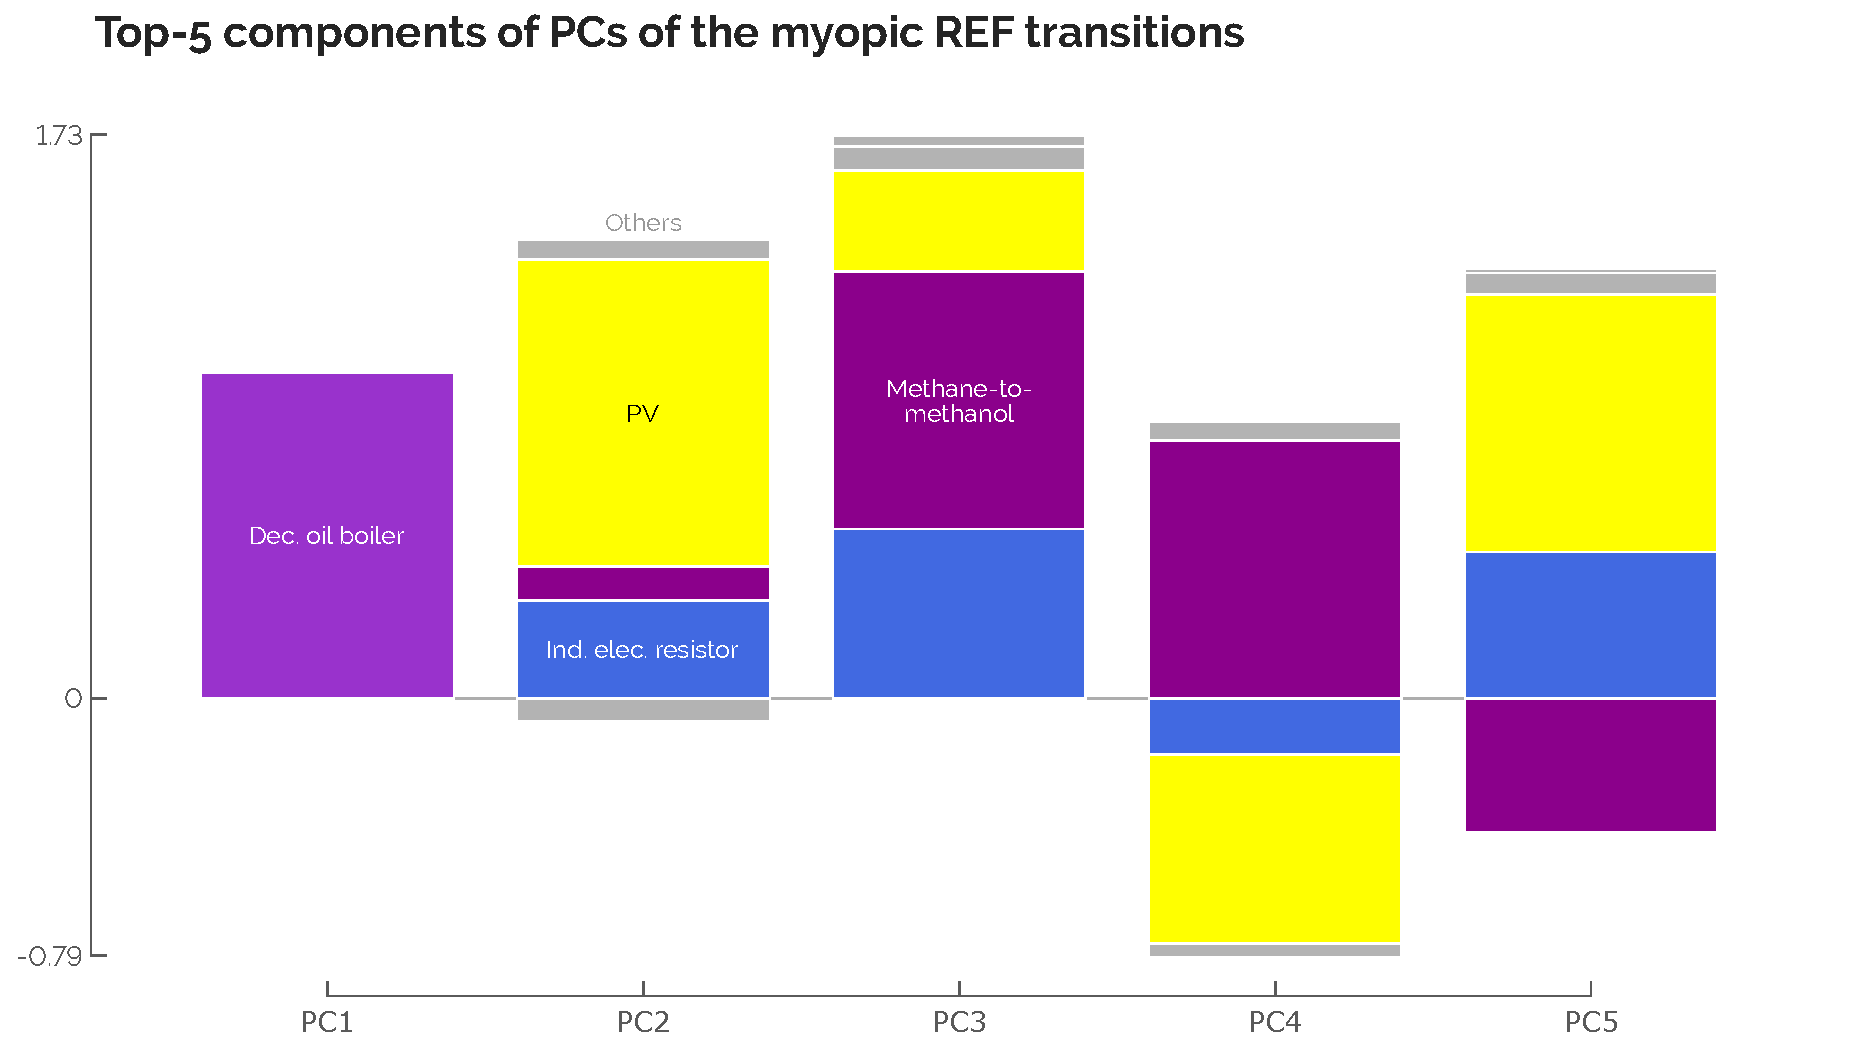
\includegraphics[width=0.75\textwidth]{Top5_PCtransition_REF_MY.pdf}
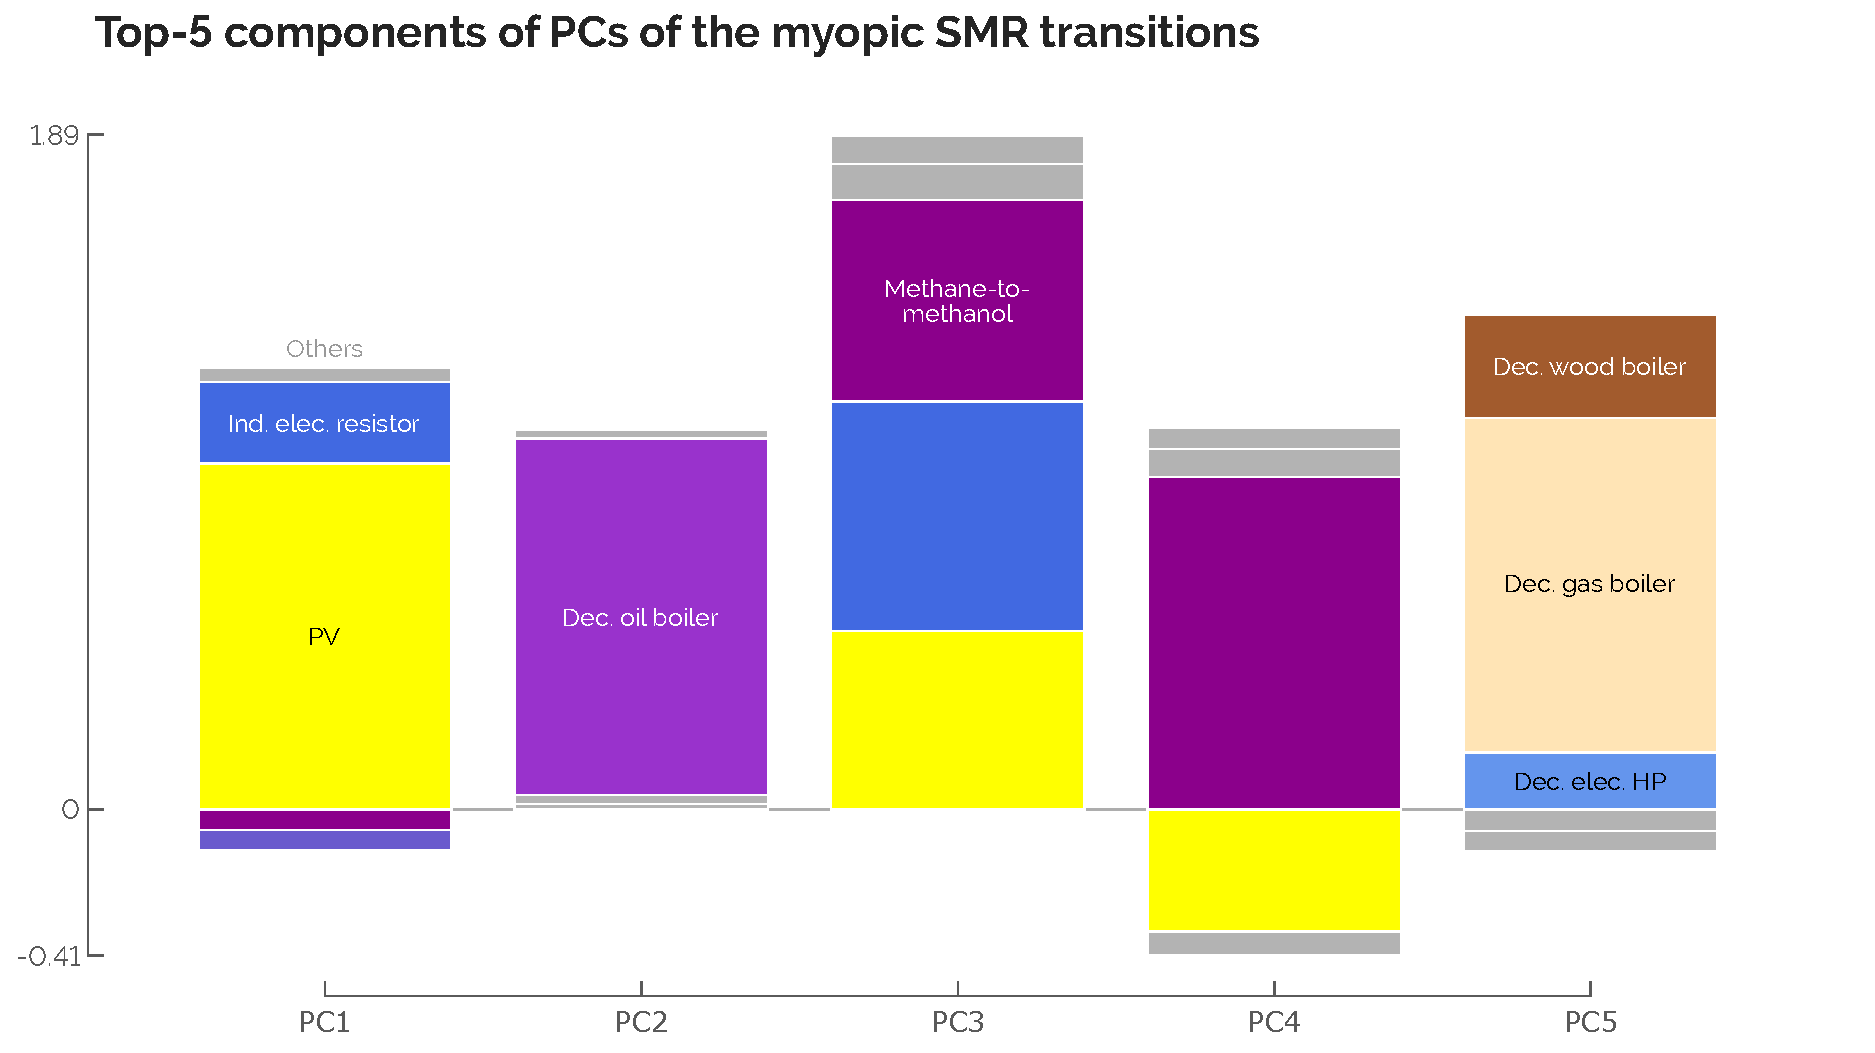
\includegraphics[width=0.75\textwidth]{Top5_PCtransition_SMR_MY.pdf}
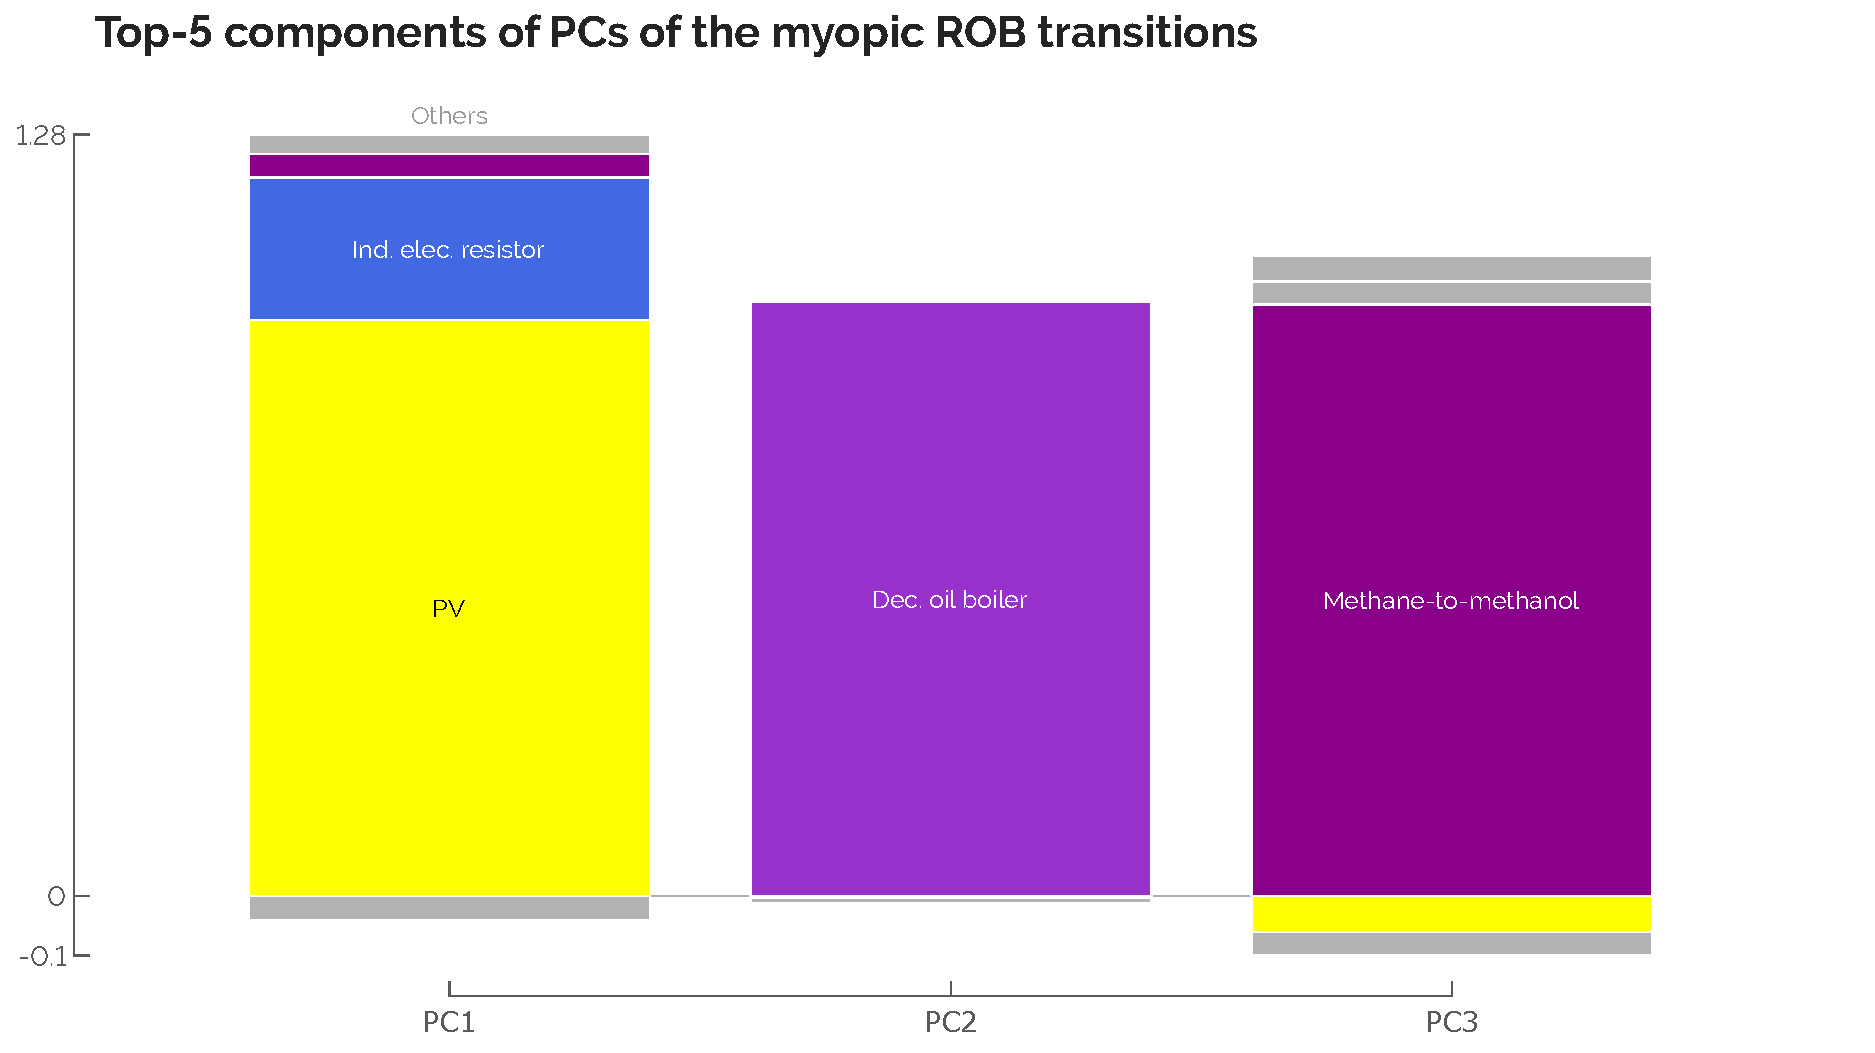
\includegraphics[width=0.75\textwidth]{Top5_PCtransition_ROB_MY.pdf}
\caption{Contribution of the top-5 technologies to the \gls{PCs} of myopic transitions for the REF, SMR and ROB cases. The variation of \gls{PV}, industrial electric resistors and \gls{LT}-heat technologies still have a major contribution of the variation in the system roadmaps. At the early stages of the myopic transitions, the installation methane-to-methanol is also subject to significant variations.}
\label{fig:Top5_PCtransition_cases}
\end{figure}

\subsection{What about the costs over the transition?}
\label{subsec:RobPol:costs_comparison}
Besides the additional capacities needed through the myopic transitions, this section takes a step back to assess the variations of costs over the transition: the total transition cost, the cumulative \gls{OPEX} by 2050 and the cumulative \gls{CAPEX} by 2050 (see Figure \ref{fig:Total_Opex_Capex_REF_ROB}). We observe that the differences are marginal. This validates the initial rationale to go beyond these costs to assess the robustness of roadmaps.

\begin{figure}[!htbp]
\centering
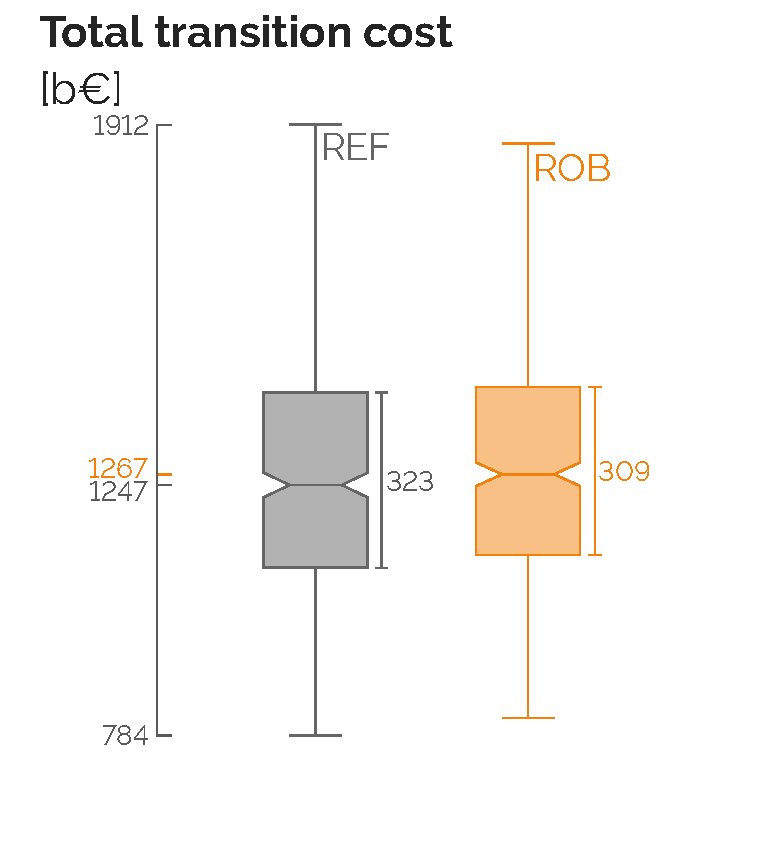
\includegraphics[width=0.325\textwidth]{Transition_cost_REF_ROB.pdf}
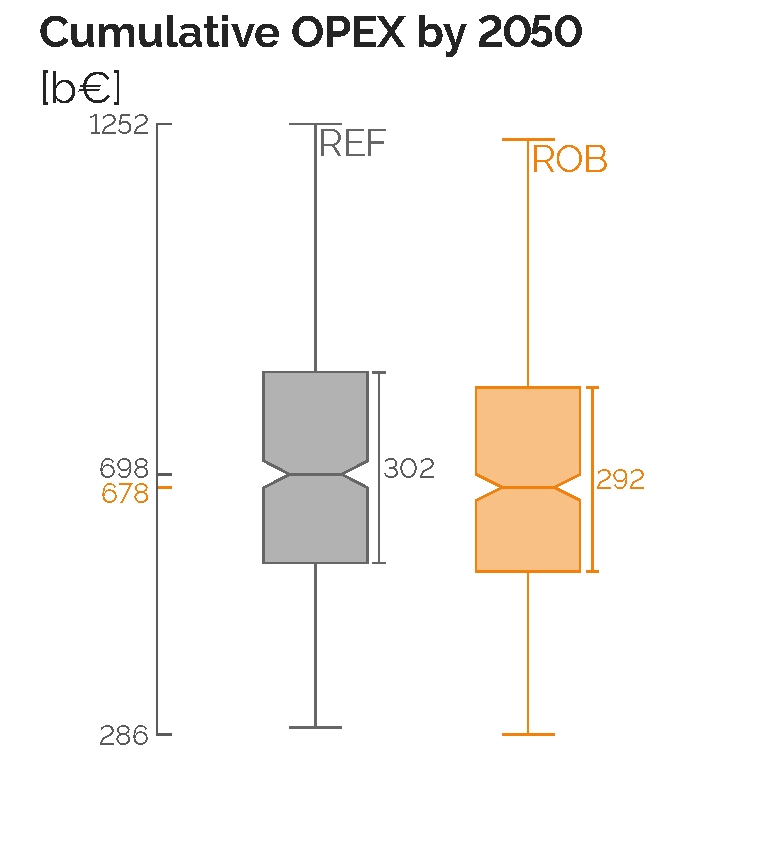
\includegraphics[width=0.325\textwidth]{OPEX_2050_REF_ROB.pdf}
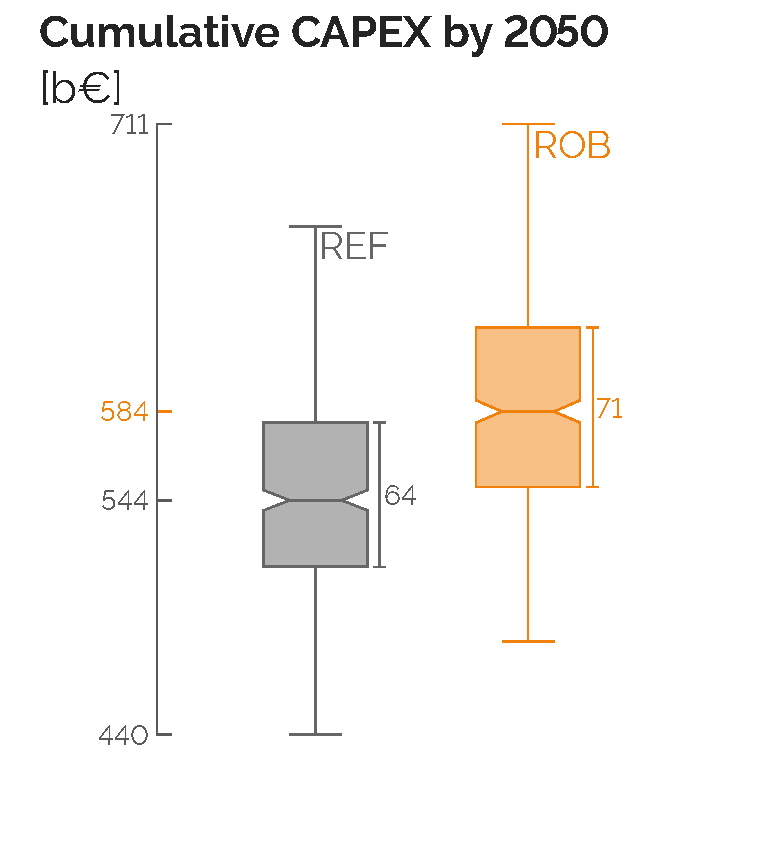
\includegraphics[width=0.325\textwidth]{CAPEX_2050_REF_ROB.pdf}
\caption{Comparison of total transition cost (left), cumulative OPEX (center) and CAPEX (right) by 2050 from the REF and ROB myopic transitions. The differences are marginal. However, the ROB roadmap lead to cheaper and less varying total transition cost. Requiring more investments at earlier stages, this roadmap is less affected by the variation of the operational costs.}
\label{fig:Total_Opex_Capex_REF_ROB}
\end{figure}

Considering the median values, the ROB roadmap leads to a 1.6\% more expensive total transition. This comes from the earlier investments in \gls{PV} panels together with electrified solutions in the heating sector that need to be renewed before the end of the transition. The extra-\gls{CAPEX} also comes from more efficient (and more expensive) technologies such as \gls{CHP}. These decisions allow being less affected by the variation of the cumulative operational costs that are dominated ($\sim$\,70\%) by the cost of purchasing energy carriers.  This makes the investment-to-operation ratio slightly higher for the ROB case (46\%) than for the REF case (44\%). 

We can assess the variation of these costs with the quartile coefficient of dispersion. This coefficient of dispersion is defined as $\left(Q_3-Q_1 \right)/\left(Q_3+Q_1 \right)$ where $Q_1=P_{25}$ and $Q_3=P_{75}$ are the first and third quartiles of the data, respectively. We observe that the ROB case has a smaller quartile coefficient of dispersion for the total transition cost and cumulative \gls{OPEX} but higher for the cumulative \gls{CAPEX} (see Table \ref{tab:quartile_coeff_dispersion}).The biggest decrease of these coefficients of dispersion between the REF and the ROB cases concerns the total transition cost. This means that the ROB case ensures to decrease more the uncertainty on this cost. 



\begin{table}[htbp!]
\caption{Quartile coefficient of dispersion for the total transition cost, cumulative OPEX and CAPEX by 2050 from the REF and ROB myopic transitions. The ROB case leads to more certain total transition cost and cumulative \gls{OPEX} than the REF case.}
\label{tab:quartile_coeff_dispersion}
\centering
\begin{tabular}{l| c c}
\toprule
\textbf{Quartile coefficient of dispersion} &  REF  & ROB \\
\midrule
Total transition cost & 12.9\% & 12.2\%  \\
Cumulative \gls{OPEX} by 2050 & 21.3\% & 21.1\% \\
Cumulative \gls{CAPEX} by 2050 & 5.9\% & 6.0\%\\
\bottomrule							
\end{tabular}
\end{table}

All these conclusions are similar to the ones observed on the study of overcapacity of \citet{moret2020overcapacity}). Working on the snapshot model and fixing the installed capacities only in the power sector, they although observed bigger gain to opt for a robust strategy rather than the deterministic solution.

\newpage
\section{Conclusions}
\label{sec:RobPol:Conclusions}
In this chapter, we applied the \gls{PCA}-based approach detailed in Chapter \ref{chap:chap_methodo} to assess the robustness of different transition roadmaps for the case of Belgium. First, starting from the principal components of each representative year, we have computed the PCs of the transition to serve as robustness metric. This showed that the variation of installed capacities of \gls{PV}, industrial electric resistors and \gls{LT}-heat technologies drove the major share (75\%) of the variation of the transition design strategy.  

Then, we have tested three roadmaps resulting from different perfect foresight optimisations: REF, SMR and ROB. Where the first two have been broadly discussed in Chapter \ref{chap:atom_mol}, the ``robust'' (ROB) case was considering the worst value of the uncertain parameters impacting the most the total transition cost following the same approach as \citet{Moret2017PhDThesis}. From these roadmaps setting the minimal installed capacities over the transition, we have assessed the variation of the additional capacities needed in myopic optimisations subject to uncertainties. This showed that counting on the installation of \gls{SMR} by 2040 was providing the same level of robustness as the reference case in the key directions of variation. However, the robust (ROB) investment roadmap --- which, in our case, anticipates the full deployment of local \gls{VRES} and the integration of efficient technologies --- is more robust than the reference scenario. Even though this roadmap represents 7.4\% more cumulative \gls{CAPEX} over the transition than the REF case, it provides more robustness towards the variations of \gls{PV} supported by the electrification of \gls{HT} and \gls{LT} heating sectors (49\%) and technologies in the transport of freight (33\%).  On top of decreasing the risk to invest into additional capacities, the ROB is also less sensitive to the variation of the costs of purchasing the energy carriers that are the main contributors of uncertainty.

Overall, this \gls{PCA}-based approach allows evaluating the variation of multiple-year transition pathway of a whole-energy system and assessing its robustness. Doing so, it brings more information than when considering only the variation of the objective function.


